\section{Betriebswirtschaftliche Analyse}
\subsection{Beschreibung möglicher Anwendungen aus Business-Sicht}

Um Faktoren und Kennzahlen für den langfristigen Erfolg des Unternehmens zu erstellen, können die Daten aus verschiedenen Perspektiven betrachtet werden. Ein mögliches Vorgehensmodell dazu bietet die Balanced-Scorecard.

Die  offensichtlichste Perspektive ist dabei die finanzielle Sicht. Zu dieser gehören verschieden traditionelle Kennzahlen wie Gewinn, Umsatz und Rentabilität. Ziele wären die Steigerung dieser oder die Identifikation und Abstoßung unrentabler Produkte. Jedoch sind die Einkaufspreise der Artikel nicht gelistet und nur deren Verkaufspreise verfügbar. Daher kann nur der reine Umsatz analysiert. Dieser wird in Abhängigkeit der Dimensionen Zeit, Produkt, Alter und Geschlecht des Kunden betrachtet. Daraus lassen sich Kennzahlen wie die monatliche Umsatzentwicklung, beliebteste und unbeliebteste Produkte und der Wert verschiedener Kundengruppen berechnen.

Ein weiterer Punkt ist die Kundenperspektive. Mögliche Ziele sind hohe Kundenzufriedenheit und ein hoher Neukundenanteil. Eine weitere Fragestellung wäre, welche Produkte von Kunden häufig zusammen gekauft werden, was auch Cross-Selling heißt. Daraus können Empfehlungen für die Kunden abgeleitet werden. Daraus abgeleitete Kennzahlen sind die Bestellungen pro Kunde und Artikel pro Bestellung

Zur Analyse und Bewertung der internen Geschäftsprozesse können die Bearbeitungszeiten der Bestellungen oder die Retouren betrachtet werden. Diese gilt es zu verringern. Außerdem kann untersucht werden, ob es bei bestimmten Produkten oder Kundengruppen zu einer Häufung von Retouren kommt.

Der vierte Punkt der Balanced-Scorecard ist Lernen und Wachstum. Dabei geht es, um die Zufriedenheit der Mitarbeiter und deren Qualifikationen. Dazu sind aber keine Daten vorhanden und eine Analyse daher nicht möglich.

\pagebreak

\subsection{Konzeptuelle Modellierung}

\subsubsection*{Retouren}
\begin{figure}[htbp] 
  \centering
     \includepdf[pages=2,pagecommand={},scale=1.05,offset=2cm 5.2cm]{phase1/adapt-diagramme.pdf}
\end{figure}

Der Retouren-Cube beinhaltet für die Retouren interessante Dimensionen. Diese sind der Grund für die Rückgabe, das Datum, das Produkt und die Altersgruppe. Darüber kann untersucht werden, welche Gründe häufig zur Retoure führen, wann gehäuft Retouren auftreten, welche Produkte zurückgegeben werden und wie sich verschiedene Altersgruppen verhalten. So können häufig reklamierte Produkte herausgefunden und aus dem Angebot entfernt werden.

\vspace{11cm}

\subsubsection*{Cross-Selling}
\begin{figure}[htbp] 
  \centering
     \includepdf[pages=4,pagecommand={},scale=1.1,offset=2cm -10.2cm]{phase1/adapt-diagramme.pdf}
\end{figure}

Der Cube Cross-Selling soll die zeitliche Entwicklung von zusammen gekauften Produkten enthalten.  Auf Basis der Ergebnisse dieser Untersuchung können beispielsweise besondere Angebote oder Produktkombinationen erstellt werden, um so den Umsatz pro Bestellung zu erhöhen.

\subsubsection*{Bestellungen}
\begin{figure}[htbp] 
  \centering
     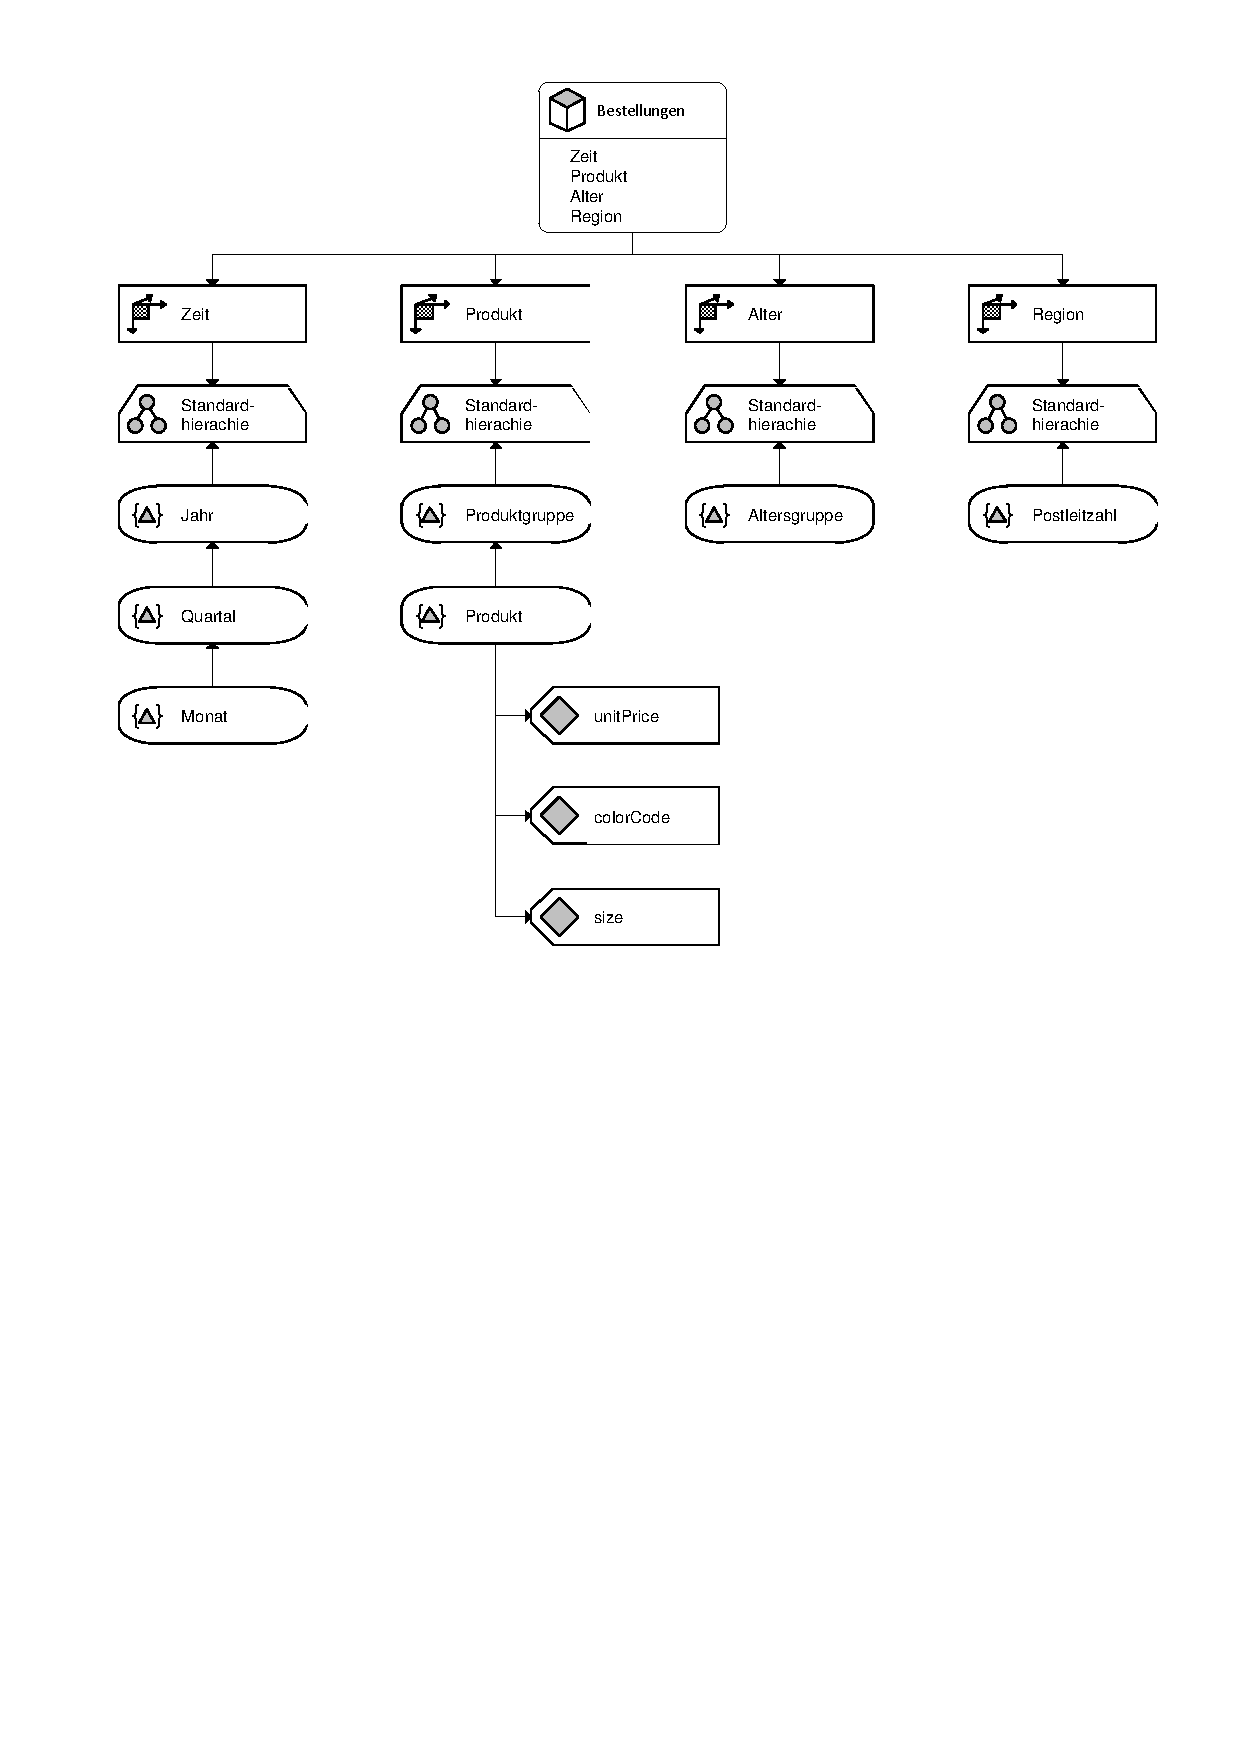
\includepdf[pages=1,pagecommand={},scale=0.8,offset=0cm 0.5cm]{phase1/adapt-diagramme.pdf}
\end{figure}

Im Cube Bestellungen soll die Anzahl der Bestellungen in Abhängigkeit von Zeit, Produkt, Newsletter-Abonnement, Altersgruppe und Herkunft der Kunden betrachtet werden. Daraus kann ermittelt werden, welche Produkte am häufigsten oder seltensten gekauft werden. Außerdem kann über den Verkaufspreis die Umsatzentwicklung berechnet werden. In Kombination mit den Altersgruppen und Regionen können wertvolle Zielgruppen bestimmt werden. In Kombination mit der Newsletterbestellung kann der durchschnittliche Umsatz von Kunden mit und ohne Newsletter untersucht werden und somit der Erfolg von diesem.

\pagebreak

\subsection{Datenverarbeitungsanforderungen}

Da als Datenquelle die operative Datenbank des Online-Shop dient, stellt diese bezogen auf die Granularität, die Aktualität und die Glaubwürdigkeit eine ausreichend hohe Datenqualität bereit.
Für weiterführende Analysen bezüglich des Gewinns oder der Rentabilität sind die Daten der Datenbank jedoch nicht ausreichend, da Informationen über Einkaufspreise und Ähnliches nicht zur Verfügung stehen. Hierfür müssten externe Datenquellen, wie Preislisten von Großhändlern, in den Analyseprozess integriert werden.

Für das Auslesen der Basisdaten bietet sich eine periodische Extraktion an, da der Fokus bei den Analysen auf der zeitlichen Entwicklung bzw. Verteilung der festgelegten Kennzahlen liegt.
Da in der Zeit-Dimension der Monat die kleinste Konsolidierungsstufe bildet, genügt es die Datenextraktion und Auswertung ein- bis zweimal im Monat durchzuführen.
